\documentclass[border=6pt]{standalone}
\usepackage{tikz}
\usepackage{pgfplots}
\pgfplotsset{compat=1.18}
\usetikzlibrary{arrows.meta,positioning,shapes.geometric,fit,backgrounds,calc,decorations.pathreplacing,patterns,pgfplots.groupplots}
\tikzset{
  blk/.style={rectangle, rounded corners=2pt, draw=black!70, thick, fill=blue!6,
              minimum height=8mm, minimum width=20mm, align=center, font=\small},
  io/.style={rectangle, rounded corners=6pt, draw=black!70, thick, fill=green!8,
             minimum height=8mm, align=center, font=\small},
  proc/.style={rectangle, draw=black!70, thick, fill=orange!10, minimum height=8mm,
               align=center, font=\small},
  dec/.style={diamond, aspect=2, draw=black!70, thick, fill=yellow!15, align=center, font=\footnotesize},
  warnbox/.style={rectangle, rounded corners=2pt, draw=red!60!black, thick, fill=red!7,
                  minimum height=8mm, align=center, font=\small},
  oklbox/.style={rectangle, rounded corners=2pt, draw=green!45!black, thick, fill=green!8,
                 minimum height=8mm, align=center, font=\small},
  ar/.style={-{Latex[length=2mm]}, thick},
  arl/.style={-{Latex[length=2mm]}, thick, dashed, draw=black!55},
  lbl/.style={font=\footnotesize\itshape, text=black!60},
  rowlab/.style={font=\tiny, text=black!75, align=left, inner sep=0pt},
  rowval/.style={font=\scriptsize, text=black!80, inner sep=0pt},
}
\definecolor{good}{RGB}{34,139,34}
\definecolor{bad}{RGB}{178,34,34}
\definecolor{warn}{RGB}{218,165,32}
\definecolor{pesblue}{RGB}{0,45,98}
\definecolor{complete}{RGB}{30,125,79}
\definecolor{partial}{RGB}{176,106,0}
\definecolor{blocked}{RGB}{166,43,43}
\begin{document}
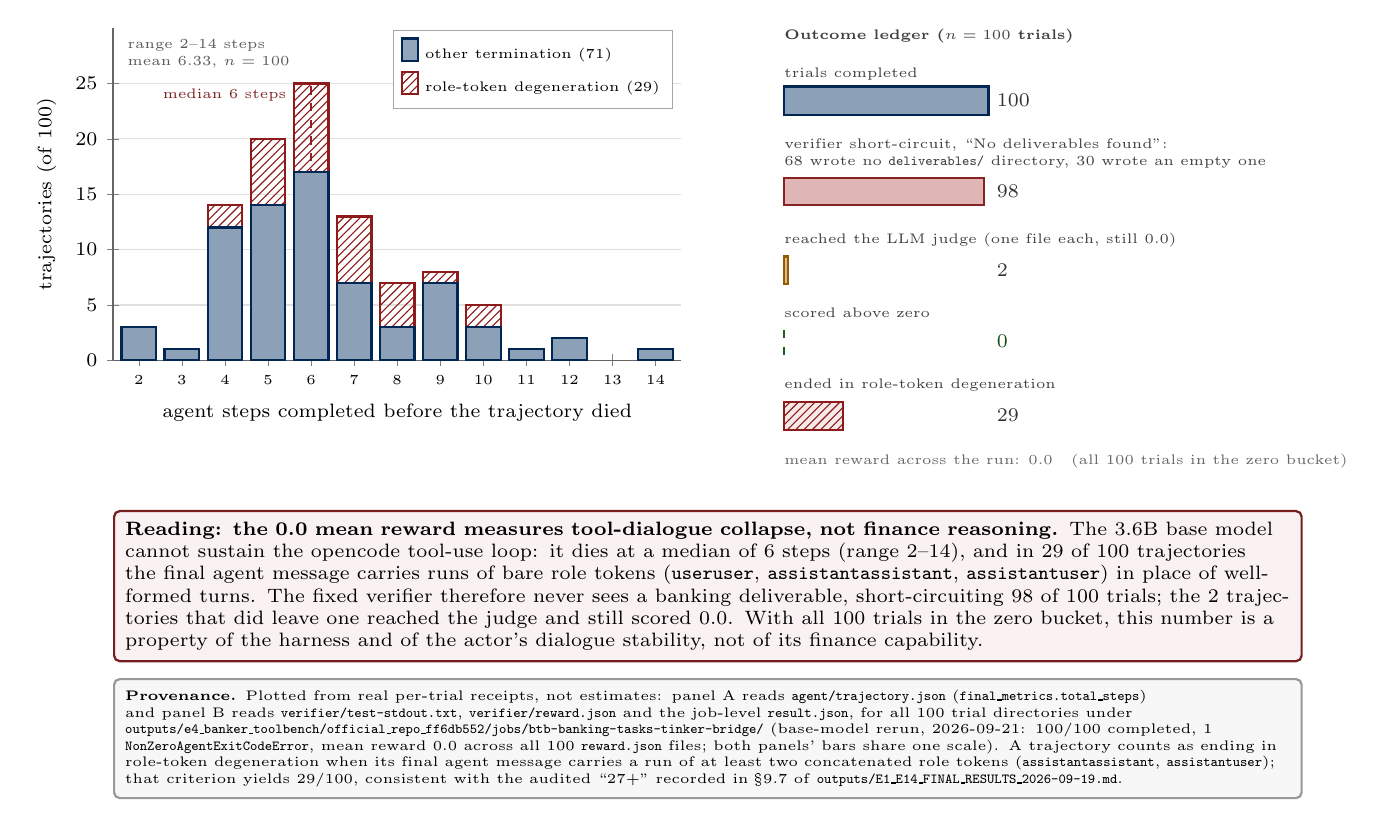
\begin{tikzpicture}

% =====================================================================
% Panel A: real per-trajectory step counts, split by terminal class.
% Data: agent/trajectory.json -> final_metrics.total_steps, all 100 trial
% directories of the 2026-09-21 base-model BankerToolBench rerun.
% totals by step: 2:3  3:1  4:14  5:20  6:25  7:13  8:7  9:8  10:5  11:1  12:2  14:1
% of which terminal role-token degeneration (the final agent message carries a
% run of >=2 concatenated role tokens, e.g. "assistantassistant"): 
%   4:2  5:6  6:8  7:6  8:4  9:1  10:2  = 29/100
% (audit E1_E14_FINAL_RESULTS_2026-09-19.md sec. 9.7 records "27+")
% =====================================================================
\begin{axis}[
  name=A,
  width=88mm, height=58mm,
  ybar stacked,
  bar width=4.4mm,
  xmin=1.4, xmax=14.6,
  ymin=0, ymax=30,
  xtick={2,3,4,5,6,7,8,9,10,11,12,13,14},
  xticklabel style={font=\tiny},
  ytick={0,5,10,15,20,25},
  yticklabel style={font=\scriptsize},
  xlabel={\scriptsize agent steps completed before the trajectory died},
  ylabel={\scriptsize trajectories (of 100)},
  label style={font=\scriptsize},
  ymajorgrids,
  grid style={black!12},
  axis lines=left,
  axis line style={black!60},
  x axis line style={-},
  y axis line style={-},
  legend style={font=\tiny, at={(0.985,0.995)}, anchor=north east, draw=black!35,
                fill=white, fill opacity=0.94, text opacity=1, row sep=1pt,
                inner sep=2.5pt, cells={anchor=west}},
  legend cell align=left,
]
% series 1 (bottom of the stack): trajectory ended some other way -- 71
\addplot+[fill=pesblue!45, draw=pesblue!85!black, thick] coordinates {
  (2,3) (3,1) (4,12) (5,14) (6,17) (7,7) (8,3) (9,7) (10,3) (11,1) (12,2) (13,0) (14,1)
};
% series 2 (top of the stack): trajectory ended in role-token degeneration -- 29
\addplot+[fill=bad!10, draw=bad!80!black, thick, pattern=north east lines,
          pattern color=bad!80!black] coordinates {
  (2,0) (3,0) (4,2) (5,6) (6,8) (7,6) (8,4) (9,1) (10,2) (11,0) (12,0) (13,0) (14,0)
};
\legend{{other termination (71)}, {role-token degeneration (29)}}
% median marker
\draw[dashed, thick, blocked!85!black] (axis cs:6,0) -- (axis cs:6,25);
\node[anchor=east, font=\tiny, text=blocked!75!black, inner sep=1pt]
  at (axis cs:5.5,24) {median 6 steps};
% span + mean, in the empty upper-left region
\node[anchor=north west, font=\tiny, text=black!65, align=left, inner sep=2pt]
  at (axis cs:1.6,29.5) {range 2--14 steps\\ mean 6.33, $n=100$};
\end{axis}

% =====================================================================
% Panel B: outcome ledger -- where the fixed evidence chain actually
% stopped. Data: verifier/test-stdout.txt + result.json, all 100 trials.
% All bars share one scale: 100 trials = 26mm.
%  100/100 completed (1 NonZeroAgentExitCodeError), mean reward 0.0
%   98/100 short-circuit: "No deliverables found ... returning score 0.0"
%         (68 wrote no deliverables/ directory, 30 wrote an empty one)
%    2/100 placed one deliverable file, reached the LLM judge, scored 0.0
%    0/100 scored above zero
%   29/100 ended in role-token degeneration (same flag as panel A)
% =====================================================================
\begin{scope}[shift={($(A.north east)+(13mm,0)$)}]
  \node[anchor=north west, font=\tiny\bfseries, text=black!75, inner sep=0pt]
    at (0,0) {Outcome ledger ($n=100$ trials)};

  % ---- row 1: trials completed
  \node[rowlab, anchor=north west] at (0,-5.0mm) {trials completed};
  \fill[pesblue!45] (0,-11.0mm) rectangle (26mm,-7.4mm);
  \draw[pesblue!85!black, thick] (0,-11.0mm) rectangle (26mm,-7.4mm);
  \node[rowval, anchor=west] at (27mm,-9.2mm) {100};

  % ---- row 2: verifier short-circuit
  \node[rowlab, anchor=north west] at (0,-14.0mm)
    {verifier short-circuit, ``No deliverables found'':\\
     68 wrote no \texttt{deliverables/} directory, 30 wrote an empty one};
  \fill[blocked!35] (0,-22.5mm) rectangle (25.48mm,-19.0mm);
  \draw[blocked!80!black, thick] (0,-22.5mm) rectangle (25.48mm,-19.0mm);
  \node[rowval, anchor=west] at (27mm,-20.7mm) {98};

  % ---- row 3: reached the judge
  \node[rowlab, anchor=north west] at (0,-26.0mm)
    {reached the LLM judge (one file each, still 0.0)};
  \fill[partial!45] (0,-32.5mm) rectangle (0.52mm,-29.0mm);
  \draw[partial!85!black, thick] (0,-32.5mm) rectangle (0.52mm,-29.0mm);
  \node[rowval, anchor=west] at (27mm,-30.7mm) {2};

  % ---- row 4: scored above zero (the null, drawn honestly)
  \node[rowlab, anchor=north west] at (0,-35.5mm) {scored above zero};
  \draw[good!70!black, thick, dashed] (0,-41.5mm) -- (0,-38.0mm);
  \node[rowval, anchor=west, text=good!55!black] at (27mm,-39.7mm) {0};

  % ---- row 5: terminal role-token degeneration (matches panel A hatch)
  \node[rowlab, anchor=north west] at (0,-44.5mm)
    {ended in role-token degeneration};
  \fill[bad!10] (0,-51.0mm) rectangle (7.54mm,-47.5mm);
  \draw[bad!80!black, thick] (0,-51.0mm) rectangle (7.54mm,-47.5mm);
  \begin{scope}
    \clip (0,-51.0mm) rectangle (7.54mm,-47.5mm);
    \fill[pattern=north east lines, pattern color=bad!80!black]
      (0,-51.0mm) rectangle (7.54mm,-47.5mm);
  \end{scope}
  \node[rowval, anchor=west] at (27mm,-49.2mm) {29};

  % ---- note: the headline null
  \node[rowlab, anchor=north west, text=black!60] (ledgerbot) at (0,-54.0mm)
    {mean reward across the run: 0.0 \; (all 100 trials in the zero bucket)};
\end{scope}

% =====================================================================
% Reading of the two panels
% =====================================================================
% The ledger's lowest element (ledgerbot) sits 13.75mm below panel A's south
% west edge (measured at compile time with \pgfpointanchor), so the
% explanation boxes start 19mm down, clearing it by ~5mm.
\node[rectangle, rounded corners=2pt, draw=blocked!70!black, thick, fill=blocked!6,
      font=\scriptsize, align=left, inner sep=4pt, text width=148mm, anchor=north west]
      (readbox) at ([yshift=-19mm]A.south west)
  {\textbf{Reading: the 0.0 mean reward measures tool-dialogue collapse, not finance
   reasoning.} The 3.6B base model cannot sustain the opencode tool-use loop: it dies at a
   median of 6 steps (range 2--14), and in 29 of 100 trajectories the final agent
   message carries runs of bare role tokens (\texttt{useruser},
   \texttt{assistantassistant}, \texttt{assistantuser}) in place of well-formed
   turns. The fixed verifier therefore never
   sees a banking deliverable, short-circuiting 98 of 100 trials; the 2 trajectories
   that did leave one reached the judge and still scored 0.0. With all 100 trials in
   the zero bucket, this number is a property of the harness and of the actor's
   dialogue stability, not of its finance capability.};

\node[rectangle, rounded corners=2pt, draw=black!40, thick, fill=black!3,
      font=\tiny, align=left, inner sep=4pt, text width=148mm, anchor=north west]
  at ([yshift=-2mm]readbox.south west)
  {\textbf{Provenance.} Plotted from real per-trial receipts, not estimates: panel A
   reads \texttt{agent/trajectory.json} (\texttt{final\_metrics.total\_steps}) and
   panel B reads \texttt{verifier/test-stdout.txt}, \texttt{verifier/reward.json}
   and the job-level \texttt{result.json}, for all 100 trial directories under
   \texttt{outputs/e4\_banker\_toolbench/official\_repo\_ff6db552/jobs/btb-banking-tasks-tinker-bridge/}
   (base-model rerun, 2026-09-21: 100/100 completed, 1 \texttt{NonZeroAgentExitCodeError},
   mean reward 0.0 across all 100 \texttt{reward.json} files; both panels' bars share
   one scale). A trajectory counts as ending in role-token degeneration when its
   final agent message carries a run of at least two concatenated role tokens
   (\texttt{assistantassistant}, \texttt{assistantuser}); that criterion yields
   29/100, consistent with the audited ``27+'' recorded in \S9.7 of
   \texttt{outputs/E1\_E14\_FINAL\_RESULTS\_2026-09-19.md}.};

\end{tikzpicture}
\end{document}
